% !TeX spellcheck = ru_RU
\documentclass[]{article}

\usepackage{amsmath,amssymb,amsthm,amscd,amsfonts}
\usepackage[utf8]{inputenc}
\usepackage[top=2cm, bottom=2cm]{geometry}
\usepackage{graphicx}
\usepackage[russian]{babel}

\newtheorem{defenition}{Определение}

\begin{document}
	\begin{titlepage}
		\begin{center}
			{\large Федеральное государственное бюджетное образовательное учреждение высшего образования
			<<Санкт-Петербургский Государственный университет>>}
			\vspace{1em}
			
			{\large Кафедра <<Статистического моделирования>>}
			\vspace{15em}
			
			{\bfseries{\Large Отчет по курсовой работе на тему\\ <<Задачи оценивания значимости выравнивания при помощи скрытых марковских моделей>>}}
		\end{center}
		\vspace{8em}
		\begin{flushleft}
			Выполнил:\\
			cт. группы 19.Б04-мм Власенко Даниил Владимирович\\
			Научный руководитель:\\
			к. ф.-м. н. Коробейников Антон Иванович
		\end{flushleft}
		\vspace{16em}
		\begin{center}
			Санкт-Петербург\\
			2021
		\end{center}
	\end{titlepage}

%	\newpage
%	\tableofcontents
%	\newpage
	
	\section{Введение}
		Последовательность длины $L$ "--- строка $D$ состоящая из $L$ символов алфавита $A$. Выравнивание последовательностей  "--- размещение двух или более последовательностей друг под другом таким образом, чтобы было легче увидеть их схожие участки. Например, даны последовательности ACEAAFAE и CEAFDCE, если расположить их друг под другом, то не будет ни одного совпадения соответствующих символов, но если вставить пропуск восьмого символа в первой последовательности и пропуски первого и пятого символов во второй последовательности, то мы получим 5 совпадений.
		\begin{center}
			\begin{tabular}{ccccccccc}
				A&C&E&A&A&F&A&E\\
				C&E&A&F&D&C&E\\
			\end{tabular}
		\end{center}
			\begin{center}
				\begin{tabular}{ccccccccc}
				A&C&E&A&A&F&A&—&E\\
				—&C&E&A&—&F&D&C&E\\
			\end{tabular}
		\end{center}
		Оценка выравнивания "--- действительное число $s$, отражающее сходство последовательностей. Способом построения оценки выравнивания $s$ может быть, например, увеличение оценки на 1 при совпадении символов, стоящих друг под другом, и уменьшение на $\frac{1}{2}$ при несовпадении. Тогда оценка $s$ приведенного выше выравнивания будет равна 3. Способ оценки выравнивания выбирается исходя из целей и вида выравнивания.
		
		Сходство последовательностей может отражать функциональные, структурные или эволюционные взаимосвязи объектов, которые описывают эти последовательности. Таким образом оценка выравнивание последовательностей может быть полезно в задаче определения степени родства биологических организмов путем сравнения их ДНК или РНК, нуклеотидных последовательностей, задаче анализа свойств белков, аминокислотных последовательностей, задаче распознавания речи человека или письменного языка и многих других приложениях.
		
		Выше был приведен пример попарного выравнивания двух строк, но если сходство последовательностей слабое, то через такое выравнивание может не получится идентифицировать взаимосвязь описываемых последовательностями объектов. Однако сравнение сразу трех и более последовательностей может позволить выявить эту взаимосвязь, такое выравнивание называется множественным. Проводить множественное выравнивание стандартными методами динамического программирования для попарного выравнивания [Ссылка на первую книгу Алгоритмов в биоинформатики] вычислительно неэффективно, но оказывается, что аппарат скрытых марковских моделей (СММ) позволяет эффективно решать эту задачу [Ссылка на статью по HMM][Ссылка на вторую книгу Алгоритмов в биоинформатики]. 
		
		СММ будут описаны далее, пока что зададимся следующим вопросом. Если есть множество последовательностей, описывающих взаимосвязанные объекты, имеется еще одна последовательность и была посчитана оценка выравнивания этой последовательности ко всему множеству каким-либо способом, то
		\begin{itemize}
			\item достаточно ли высокая эта оценка, чтобы считать объект, описываемый последовательностью, родственным к объектам, описываемым множеством, или шум, т.е. случайная последовательность, мог добиться такой оценки.
			\item достаточно ли низкая эта оценка, чтобы считать объект описываемый последовательностью, не родственным к объектам, описываемым множеством, или сигнал, т.е. последовательность, описывающая взаимосвязанный с множеством объект, мог получить такую оценку. 
		\end{itemize}
		Ложноположительная вероятность оценки $s$ "--- это вероятность того, что шум получит оценку равную или выше $s$. Истинноположительная вероятность оценки $s$ "--- это вероятность того, что сигнал получит оценку равную или выше $s$. 
		
		Далее будет описаны метод, который позволяет эффективно вычислять введенные выше два термина.
		
		\section{Метод}
		Сначала опишем модели, затем алгоритмы, которые используются для манипуляции ими.
		\subsection{Модели}
		Нам потребуется Профильная СММ [Ссылка на вторую книгу Алгоритмы в Биоинформатике], с помощью которой будут вычисляться оценки последовательностей, и фоновая модель, которая будет описывать шум.
		\subsubsection{Скрытые марковские модели}						
			\begin{defenition}
				Пусть $X_{n}$ и $Y_{n}$ дискретные стохастические процессы, \\$n \geq 1$. Пара $(X_{n}, Y_{n})$ называется скрытой марковской моделью, если
				\begin{itemize}
					\item $X_{n}$~--- марковский процесс, поведение которого напрямую не наблюдается ("скрытый");
					\item $P(Y_{n} = y_{n}|X_{1} = x_{1},\dots, X_{n} = x_{n}) = P(Y_{n}|X_{n}=x_{n})$ для любого $n \geq 1$, где $x_{1},\dots,x_{n}$~--- значения, принимаемые процессом  $X_{n}$ (\textbf{состояния модели}), $ y_{n}$~--- значение, принимаемое процессом $Y_{n}$ (\textbf{наблюдаемый символ модели}).
				\end{itemize}
			\end{defenition}
			
			Если для удобства реализации алгоритмов добавить специальное \textit{начальное} и специальное \textit{конечное} состояния, в которых СММ начинает и заканчивает работу и не испускает наблюдаемых символов, тогда \textit{путь} $\pi$ в СММ начинается в начальном состоянии, заканчивается в конечном состоянии и проходит от состояния к состоянию, испуская в каждом состоянии наблюдаемый символ. \textit{Последовательность} $D$ связанная с путем $\pi$ "--- последовательность наблюдаемых символов, которая была получена в результате прохода СММ по пути $\pi$.
			
			\textit{Оценка} пути $s(\pi)$ "--- вероятность пути $\pi$, то есть $s(\pi)=P(X_{n},\dots,X_{1})$.
			
			
			
			
			
	
		\begin{figure}[h]
			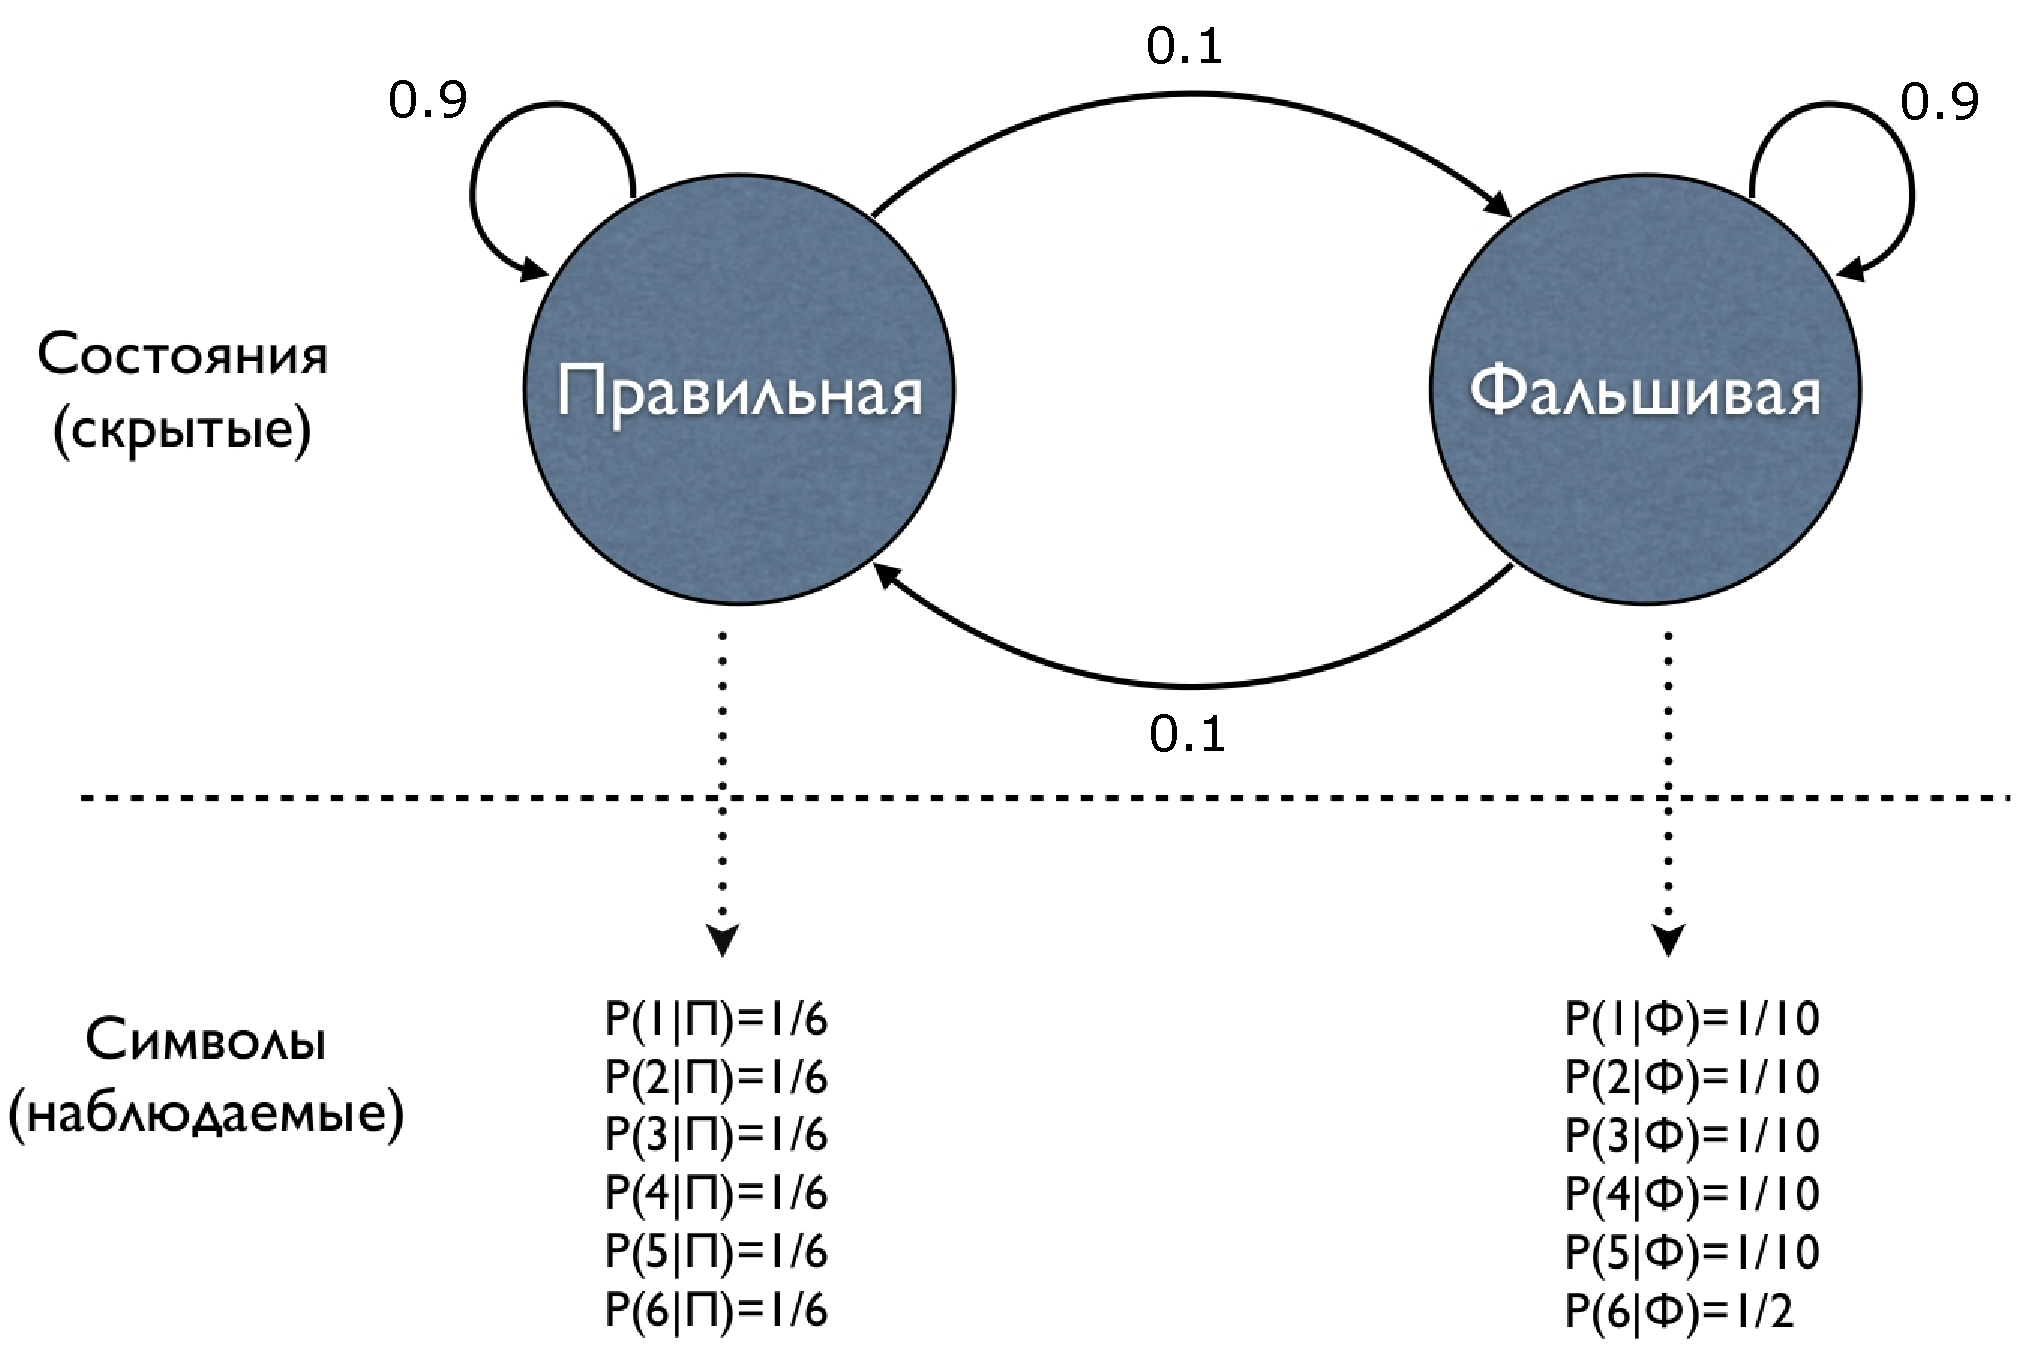
\includegraphics[width=12cm, height=8cm]{dishonestCasino}
			\centering
			\caption{Нечестное казино.}
		\end{figure}
		
		На протяжении семестра я работал с моделью <<Нечестного казино>> (рис. 1). Предположим, существует казино, которое вместе с обычной игральной костью использует нагруженную кость, которая с большей чем 1/6 вероятностью выдает определенное число. Кости могут меняться между собой с определенной вероятностью. Кости выглядят одинаково, поэтому мы не знаем, какая кость --- честная или нагруженная --- используется в определенный момент времени, но мы можем наблюдать цифры, которые выпадают раз за разом.
		
		Целью работы на семестр было ознакомление с основами скрытых марковских моделей.
		
		Все алгоритмы, используемые в курсовой работе, реализованы на языке С++ и доступны в публичном репозитории --- https://github.com/Daniil-Vlasenko/Coursework5.git.

	\subsection{Обозначения}	
		В примере выше кости являются состояниями модели, выпадающие числа~--- наблюдаемыми символами. Введем для дальнейшей работы обозначения:
		\vspace{0.5cm}\\	
		$M$ --- число состояний модели;\\
		$K$ --- число различных наблюдаемых символов;\\
		$N$ --- длина наблюдаемой последовательности;\\
		$x_{n}$ --- состояние модели в момент времени $n$;\\
		$y_{n}$ --- наблюдаемый символ в момент времени $n$;\\
		$X$ --- конечная последовательность состояний модели;\\
		$Y$ --- конечная последовательность наблюдаемых символов;\\
		$1,\dots, M$ --- состояния модели;\\
		$v_{1}, \dots, v_{K}$ --- наблюдаемые символы;\\
		$\pi = \{\pi_{i}\}, \pi_{i}=P(x_{1}=i)$ --- вероятность нахождения модели в состоянии $i \in 1, \dots, M$ в начале эксперимента, т.е. в момент времени $n=1$;\\
		$A = \{a_{ij}\}, a_{ij}=P(x_{n+1}=j|x_{n}=i)$ --- вероятность перехода модели из состояния $i \in 1, \dots, M$ в состояние $j \in 1, \dots, M$;\\
		$B = \{b_{j}(v_{k})\}, b_{j}(v_{k})=P(v_{k}|x_{n}=j)$ --- вероятность получения наблюдаемого символа $v_{k}, k \in 1,\dots, K$ в состоянии $j  \in 1, \dots, M$;\\		
		$\lambda = (A, B, \pi)$ --- скрытая марковская модель с параметрами $A, B, \pi$.\\	
		
	\section{Проделанная работа}
		На основе модели <<Нечестного казино>> и нескольких статей \cite{Dugad96,Stamp21,Jurafsky21,Rabiner89} были изучены и реализованы алгоритмы, решающие три основные задачи, к которым сводится приложение скрытых марковских моделей:
		\begin{enumerate}
			\item Дана модель $\lambda = (A, B, \pi)$, как вычислить $P(Y|\lambda)$ --- Forward--Backward процедуры.
			\item Дана модель $\lambda = (A, B, \pi)$, нужно найти последовательность состояний $X$, которая максимизирует вероятность $P(Y,X|\lambda)$ --- алгоритм Витерби.
			\item Как изменить параметры модели $\lambda = (A, B, \pi)$, чтобы максимизировать вероятность $P(Y|\lambda)$ --- алгоритм Баума"--~Велша.
		\end{enumerate}
		Алгоритмы подробно описаны в статье \cite{Dugad96}, здесь приведу краткое изложение шагов алгоритмов и результаты их работы.
		
		\subsection{Forward--Backward процедуры}
			Предположим, что нужно узнать вероятность наблюдаемой последовательности $P(Y|\lambda)$. Для этого нужно посчитать $P(Y|X,\lambda)P(X|\lambda)$ для всех возможных последовательностей состояний $X$, затем сложить результаты.
			\[
				P(Y|\lambda) = \sum_{X}{P(Y|X,\lambda)P(X|\lambda)} = \sum_{X}{\pi_{x_{1}}b_{x_{1}}(y_{1})a_{x_{1}x_{2}}b_{x_{2}}(y_{2}) \dots a_{x_{N-1}x_{N}}b_{x_{N}}(y_{N})}
			\]
			В этом уравнении происходит $2NM^N$ умножений, что при $M=5$ и $N=100$ будет означать примерно $10^{72}$ умножений, что делает такое вычисление вероятности крайне неэффективным.
		
			Forward--Backward алгоритмы полезны тем, что позволяют вычислять вероятность наблюдаемой последовательности $Y$ за $M^{2}N$ умножений вместо $2NM^N$, если считать вероятность обычным методом через сумму произведений.
			\subsubsection{Forward процедура}
				Определим forward значение $\alpha_{n}(i)$ следующим образом:
				\[
					\alpha_{n}(i) = P(y_{1}, y_{2}, \dots, y_{n}, x_{n} = i | \lambda)
				\]
				т.е. это вероятность последовательности наблюдаемых символов $Y$ до момента времени $n$, при этом в момент времени $n$ модель $\lambda$ находится в состоянии $i$. $\alpha_{n}(i)$ может быть посчитана последовательно:
				
				\begin{enumerate}
					\item \[
						\alpha_{1}(i) = \pi_{i}b_{i}(y_{1}), 1 \leq i \leq M
					\]
					\item для $n = 1,2,\dots,N-1, 1 \leq j \leq M$
					\[
						\alpha_{n+1}(j) = \left( \sum_{i=1}^{M}{\alpha_{n}(i)a_{ij}} \right) b_{j}(y_{n+1})
					\]
					\item тогда
					\[
						P(Y|\lambda) = \sum_{i=1}^{M}{\alpha_{N}(i)}
					\]
				\end{enumerate}
			\subsubsection{Backward процедура}
				Определим backward значение $\beta_{n}(i)$ следующим образом:
				\[
				\beta_{n}(i) = P(y_{n+1}, y_{n+2}, \dots, y_{N}|x_{n} = i,
				\lambda)
				\]
				т.е. это вероятность наблюдаемой последовательности $Y$ с момента времени $n+1$ до $N$, при этом в момент времени $n$ модель находится в состоянии $i$.  $\beta_{n}(i)$ считается так:
				
				\begin{enumerate}
					\item \[
					\beta_{N}(i) = 1,1 \leq i \leq M
					\]
					\item для $n = N-1, N-2,\dots,1, 1 \leq i \leq M$
					\[
					\beta_{n}(i) = \sum_{j=1}^{M}{a_{ij}b_{j}(y_{n+1})
					\beta_{n+1}(j)}
					\]
					\item тогда
					\[
					P(Y|\lambda) = \sum_{i=1}^{M}{\pi_{i}b_{i}(y_{1})\beta_{1}(i)}
					\]
				\end{enumerate}
	
		Оба алгоритма были протестированы и использованы далее в курсовой работе.
	
	\subsection{Алгоритм Витерби}
		Алгоритм Витерби позволяет найти последовательность состояний $X^{*}$, которая максимизирует вероятность появления данной наблюдаемой последовательности $P(Y,X|\lambda)$, т.е $X^{*} = \arg \max_{X} P(Y,X|\lambda)$.
		\begin{enumerate}
			\item Инициализация. Для $1 \leq i \leq M$
			\[
				\delta_{1}(i) = \pi_{i}b_{i}(y_{1})
			\]
			\[
				\psi_{1}(i) = 0
			\]
			\item Рекурсивное вычисление. Для $2 \leq n \leq N$ для $1 \leq j \leq M$
			\[
				\delta_{n}(j) = \max_{1 \leq i \leq M}(\delta_{n-1}(i)a_{ij})b_{j}(y_{n})
			\]
			\[
				\psi_{n}(j) = \arg \max_{1 \leq i \leq M} (\delta_{n-1}(i)a_{ij})
			\]
			\item Прерывание алгоритма
			\[
				P^{*} = \max_{1 \leq i \leq M} (\delta_{N}(i))
			\]
			\[
				q^{*}_{N} = \arg \max_{1 \leq i \leq M} (\delta_{N}(i))
			\]
			\item Восстановление оптимальной последовательности состояний. Для $n = N-1, N-2, \dots, 1$
			\[
				q^{*}_{n} = \psi_{n+1}(q^{*}_{n+1})
			\]
		\end{enumerate}
	
	Продемонстрирую работу алгоритма. Предположим, дана наблюдаемая последовательность $Y = 1315455312545412355311134313154553125434123 15515\\53433144513122454123555155343$. Тогда последовательность состояний $X^{*}$, максимизирующая $P(Y,X|\lambda)$ для модели указанной на рисунке 1, будет $0001111111\\1111111111111110000111111111111000111111111111111000011100111111111$.
	
	
	\subsection{Алгоритм Баума"--~Велша}
		Данный алгоритм позволяет изменять параметры $\lambda$ так, чтобы максимизировалась вероятность появления заданной наблюдаемой последовательности $P(Y|\lambda)$. Предполагается, что известны некоторые начальные параметры модели $\lambda$. Для его реализации потребуется объявить две вспомогательные функции. Определим $\gamma_{n}(i)$:
		\[
			\gamma_{n}(i) = P(x_{n} = i, Y|\lambda) = \frac{P(x_{n}=i, Y|\lambda)}{P(Y|\lambda)} = \frac{\alpha_{n}(i)\beta_{n}(i)}{P( Y|\lambda)}
		\]
		т.е. это вероятность того, что в момент времени $n$ модель будет находиться в состоянии $i$. Следовательно, сумма этих значений для конкретного $i$ от $n=0$ до $n=N$ будет представлять собой ожидаемое число посещений моделью состояния $i$.
		
		Определим $\xi_{n}(i,j)$:
		\begin{multline*}
			\xi_{n}(i,j) = P(x_{n} = i, x_{n+1} = j | Y, \lambda) = \frac{P(x_{n} = i, x_{n+1} = j, Y | \lambda)}{P(Y | \lambda)} =\\= \frac{\alpha_{n}(i)a_{ij}b_{j}(y_{n+1})\beta_{n+1}(j)}{P(Y|\lambda)}
		\end{multline*}
		т.е. это вероятность того, что модель в момент времени $n$ будет находиться в состоянии $i$, а в момент времени $n+1$ в состоянии $j$. Тогда сумма от $n=0$ до $n=N-1$ для конкретных $i$ и $j$ будет означать ожидаемое число переходов модели из состояния $i$ в состояние $j$.
		
		Теперь можно определить формулы переоценки параметров Баума"--~Велша, которые будут изменять параметры модели так, чтобы вероятность появления заданной наблюдаемой последовательности $P(Y|\lambda)$ увеличивалась: 
		\[
			\hat{\pi}_{i} = \gamma_{n}(i), 1 \leq i \leq M
		\]
		\[
			\hat{a}_{ij} = \sum_{n=1}^{N-1}{\xi_{n}(i,j)} \left/ \sum_{n=1}^{N-1}{\gamma_{n}(i)} \right.
		\]
		\[
			\hat{b}_{j}(v_{k}) = \sum_{n=1, y_{n}=v_{k}}^{N}{\gamma_{n}(i)} \left/ \sum_{n=1}^{N}{\gamma_{n}(i)} \right.
		\] 
		Если повторять описанные выше вычисления для моделей с новыми параметрами раз за разом, то функция вероятности $P(Y|\lambda)$ будет сходиться к своему экстремальному значению. 
		
		Оказывается, что начальные параметры модели очень важны, так как алгоритм может сходиться к локальным экстремумам, что приводит к неверным результатам.
		
		\subsubsection{Начальные параметры алгоритма Баума"--~Велша}
			Предположим, что дана модель <<Нечестного казино>> $\lambda$, которая приводилась на рисунке 1. Мы хотим выяснить вероятностные параметры $\pi, A, B$ модели $\lambda$. Для этого понадобится задать априорные параметры для модели $\lambda$, которые очень важны для результата. 
			
			Пусть честная кость "--- это состояние 1, нагруженная кость "--- состояние 2. Ясно, что честная кость будет выдавать результаты от 1 до 6 с вероятностью $1/6$, т.е. $b_{1}(v_{k}) = 1/6, v_{k}=1,\dots,6$. Вероятность 6 для нагруженной кости $b_{2}(6)$ может быть посчитана как частота, с которой 6 встречается в наблюдаемой последовательности, умноженная на 2. Тогда $b_{2}(v_{k}) = 1 - b_{2}(6)/5, v_{k}=1,\dots,5$. Начальное распределение состояний не сильно влияет на результаты, поэтому можно задать его так $\pi = (0.5, 0.5)$. Осталось разобраться с параметрами переходов. 
			
			Нарисуем график функции вероятности $P(Y|\lambda)$ от значения параметра перехода состояния в себя (пусть эти параметры будут одинаковые для обоих состояний) (рис. 2). Такая функция называется функцией правдоподобия. Априорное значение 0.928 для перехода в себя наиболее подходящее, вычисления демонстрирует график, значит начнем с него.
			
			\begin{figure}[h]
				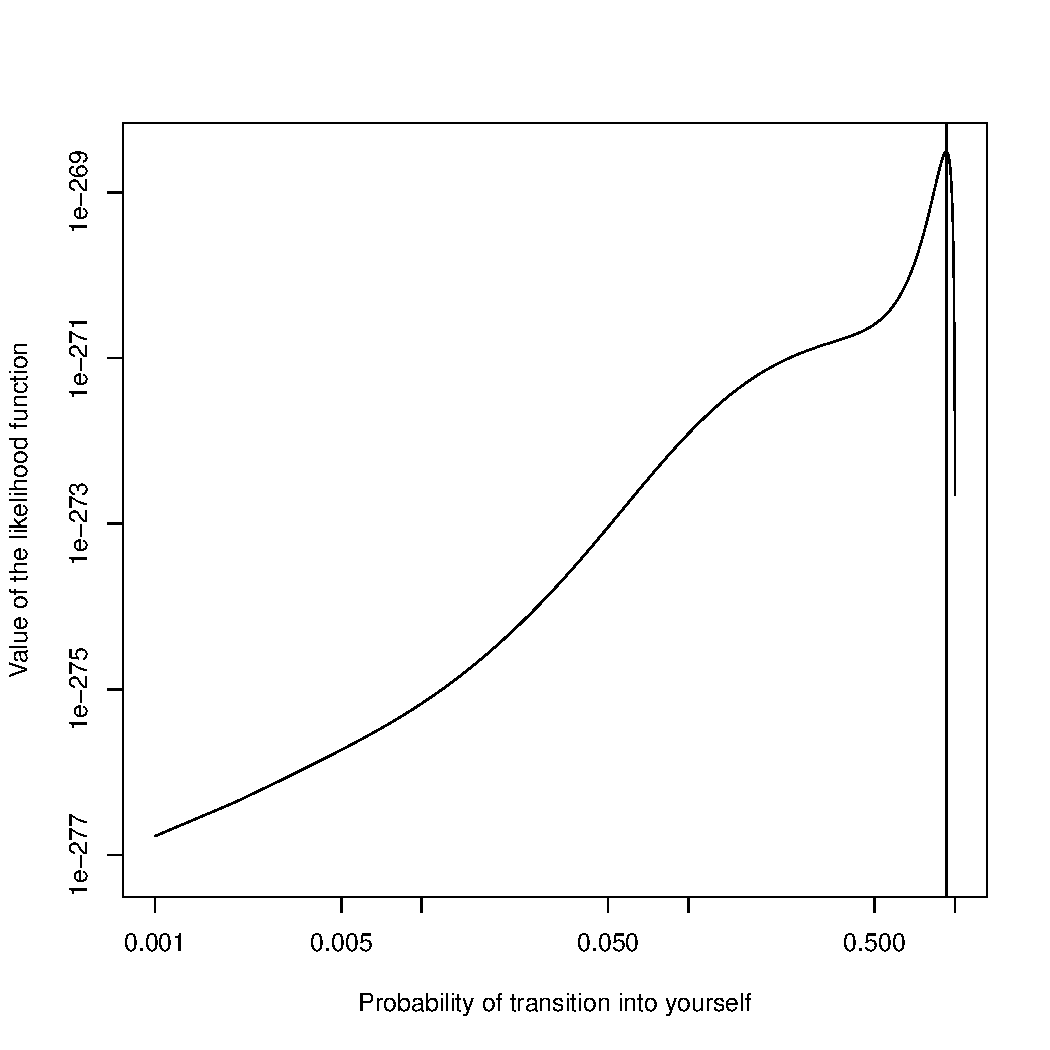
\includegraphics[width=12cm, height=12cm]{Dependence of the likelihood function on transition probability log}
				\centering
				\caption{Зависимость функции правдоподобия от вероятности перехода состояния в себя}
			\end{figure}
			
			Алгоритм сходится к определенным параметрам, повторим вычисления 100 раз и найдем среднее для параметров. Получаем, что 
			\[
				\bar{\pi} = (0.71041, 0.28959)
			\]
			\[
			\bar{A} = 
			\begin{pmatrix}
				0.915482 & 0.084518\\
				0.141648 & 0.858352
			\end{pmatrix}
			\]
			\[
			\bar{B}	=
			\begin{pmatrix}
				0.166206 & 0.166292 & 0.166868 & 0.162564 & 0.164274 & 0.173797\\ 
				0.084606 & 0.084335 & 0.084714 & 0.082356 & 0.083339 & 0.580647 
			\end{pmatrix}
			\]				
			Дисперсия результатов алгоритма:
			\[
			D(\pi) = (0.038035, 0.038035)
			\]
			\[
			D(A) = 
			\begin{pmatrix}
				0.000111 & 0.000111\\
				0.000058 & 0.000058
			\end{pmatrix}
			\]
			\[
			D(B) =
			\begin{pmatrix}
				0.000506 & 0.000503 & 0.000538 & 0.000604& 0.000568 & 0.000003\\ 
				0.000387 & 0.00047 & 0.000418 & 0.000411 & 0.000374 & 0.007149 
			\end{pmatrix}
			\]
	
	\section{Дальнейшая работа}	
		Дальше предстоит изучить методы выравнивания последовательностей, методы оценивания выравнивания последовательностей и обобщить имеющиеся знания об оценивании выравнивания для классических профильных скрытых марковских моделей на альтернативные классы скрытых марковских моделей, часто встречающихся в задачах биоинформатики.  
		
	\section{Литература}
	\renewcommand{\refname}{}
	\vspace{-25pt}
	\bibliographystyle{ugost2008mod}
	\bibliography{references}
			
		
		

	
	
	
	
	
	
	
\end{document}